\documentclass[twoside]{book}

% Packages required by doxygen
\usepackage{fixltx2e}
\usepackage{calc}
\usepackage{doxygen}
\usepackage[export]{adjustbox} % also loads graphicx
\usepackage{graphicx}
\usepackage[utf8]{inputenc}
\usepackage{makeidx}
\usepackage{multicol}
\usepackage{multirow}
\PassOptionsToPackage{warn}{textcomp}
\usepackage{textcomp}
\usepackage[nointegrals]{wasysym}
\usepackage[table]{xcolor}

% Font selection
\usepackage[T1]{fontenc}
\usepackage[scaled=.90]{helvet}
\usepackage{courier}
\usepackage{amssymb}
\usepackage{sectsty}
\renewcommand{\familydefault}{\sfdefault}
\allsectionsfont{%
  \fontseries{bc}\selectfont%
  \color{darkgray}%
}
\renewcommand{\DoxyLabelFont}{%
  \fontseries{bc}\selectfont%
  \color{darkgray}%
}
\newcommand{\+}{\discretionary{\mbox{\scriptsize$\hookleftarrow$}}{}{}}

% Page & text layout
\usepackage{geometry}
\geometry{%
  a4paper,%
  top=2.5cm,%
  bottom=2.5cm,%
  left=2.5cm,%
  right=2.5cm%
}
\tolerance=750
\hfuzz=15pt
\hbadness=750
\setlength{\emergencystretch}{15pt}
\setlength{\parindent}{0cm}
\setlength{\parskip}{3ex plus 2ex minus 2ex}
\makeatletter
\renewcommand{\paragraph}{%
  \@startsection{paragraph}{4}{0ex}{-1.0ex}{1.0ex}{%
    \normalfont\normalsize\bfseries\SS@parafont%
  }%
}
\renewcommand{\subparagraph}{%
  \@startsection{subparagraph}{5}{0ex}{-1.0ex}{1.0ex}{%
    \normalfont\normalsize\bfseries\SS@subparafont%
  }%
}
\makeatother

% Headers & footers
\usepackage{fancyhdr}
\pagestyle{fancyplain}
\fancyhead[LE]{\fancyplain{}{\bfseries\thepage}}
\fancyhead[CE]{\fancyplain{}{}}
\fancyhead[RE]{\fancyplain{}{\bfseries\leftmark}}
\fancyhead[LO]{\fancyplain{}{\bfseries\rightmark}}
\fancyhead[CO]{\fancyplain{}{}}
\fancyhead[RO]{\fancyplain{}{\bfseries\thepage}}
\fancyfoot[LE]{\fancyplain{}{}}
\fancyfoot[CE]{\fancyplain{}{}}
\fancyfoot[RE]{\fancyplain{}{\bfseries\scriptsize Generated by Doxygen }}
\fancyfoot[LO]{\fancyplain{}{\bfseries\scriptsize Generated by Doxygen }}
\fancyfoot[CO]{\fancyplain{}{}}
\fancyfoot[RO]{\fancyplain{}{}}
\renewcommand{\footrulewidth}{0.4pt}
\renewcommand{\chaptermark}[1]{%
  \markboth{#1}{}%
}
\renewcommand{\sectionmark}[1]{%
  \markright{\thesection\ #1}%
}

% Indices & bibliography
\usepackage{natbib}
\usepackage[titles]{tocloft}
\setcounter{tocdepth}{3}
\setcounter{secnumdepth}{5}
\makeindex

% Hyperlinks (required, but should be loaded last)
\usepackage{ifpdf}
\ifpdf
  \usepackage[pdftex,pagebackref=true]{hyperref}
\else
  \usepackage[ps2pdf,pagebackref=true]{hyperref}
\fi
\hypersetup{%
  colorlinks=true,%
  linkcolor=blue,%
  citecolor=blue,%
  unicode%
}

% Custom commands
\newcommand{\clearemptydoublepage}{%
  \newpage{\pagestyle{empty}\cleardoublepage}%
}

\usepackage{caption}
\captionsetup{labelsep=space,justification=centering,font={bf},singlelinecheck=off,skip=4pt,position=top}

%===== C O N T E N T S =====

\begin{document}

% Titlepage & ToC
\hypersetup{pageanchor=false,
             bookmarksnumbered=true,
             pdfencoding=unicode
            }
\pagenumbering{alph}
\begin{titlepage}
\vspace*{7cm}
\begin{center}%
{\Large Vectorial\+\_\+\+O\+D\+E\+\_\+\+Solver }\\
\vspace*{1cm}
{\large Generated by Doxygen 1.8.14}\\
\end{center}
\end{titlepage}
\clearemptydoublepage
\pagenumbering{roman}
\tableofcontents
\clearemptydoublepage
\pagenumbering{arabic}
\hypersetup{pageanchor=true}

%--- Begin generated contents ---
\chapter{Hierarchical Index}
\section{Class Hierarchy}
This inheritance list is sorted roughly, but not completely, alphabetically\+:\begin{DoxyCompactList}
\item exception\begin{DoxyCompactList}
\item \contentsline{section}{dimnotmatch}{\pageref{classdimnotmatch}}{}
\item \contentsline{section}{ordernotmatch}{\pageref{classordernotmatch}}{}
\item \contentsline{section}{timesteppossitive}{\pageref{classtimesteppossitive}}{}
\end{DoxyCompactList}
\item \contentsline{section}{O\+D\+E\+\_\+\+System}{\pageref{class_o_d_e___system}}{}
\begin{DoxyCompactList}
\item \contentsline{section}{Adams\+\_\+\+Bashforth\+\_\+\+System}{\pageref{class_adams___bashforth___system}}{}
\item \contentsline{section}{Forward\+Euler\+\_\+\+System}{\pageref{class_forward_euler___system}}{}
\item \contentsline{section}{R\+K\+System4th\+\_\+\+System}{\pageref{class_r_k_system4th___system}}{}
\end{DoxyCompactList}
\item \contentsline{section}{Reader}{\pageref{class_reader}}{}
\begin{DoxyCompactList}
\item \contentsline{section}{Data\+\_\+\+Reader}{\pageref{class_data___reader}}{}
\begin{DoxyCompactList}
\item \contentsline{section}{Matrix\+\_\+\+Reader}{\pageref{class_matrix___reader}}{}
\item \contentsline{section}{Vector\+\_\+\+Reader}{\pageref{class_vector___reader}}{}
\end{DoxyCompactList}
\item \contentsline{section}{function\+\_\+reader}{\pageref{classfunction__reader}}{}
\item \contentsline{section}{Setting\+\_\+\+Reader}{\pageref{class_setting___reader}}{}
\end{DoxyCompactList}
\item \contentsline{section}{Setting}{\pageref{struct_setting}}{}
\end{DoxyCompactList}

\chapter{Class Index}
\section{Class List}
Here are the classes, structs, unions and interfaces with brief descriptions\+:\begin{DoxyCompactList}
\item\contentsline{section}{\mbox{\hyperlink{class_adams___bashforth___system}{Adams\+\_\+\+Bashforth\+\_\+\+System}} \\*Inheritance of class \mbox{\hyperlink{class_o_d_e___system}{O\+D\+E\+\_\+\+System}}\+: Solving the vectorial system by means of Adams Bashforth method }{\pageref{class_adams___bashforth___system}}{}
\item\contentsline{section}{\mbox{\hyperlink{class_data___reader}{Data\+\_\+\+Reader}} \\*Inheritance of class \mbox{\hyperlink{class_reader}{Reader}} which specializes in reading data from files }{\pageref{class_data___reader}}{}
\item\contentsline{section}{\mbox{\hyperlink{classdimnotmatch}{dimnotmatch}} \\*Inheritance of class exception\+: deal with dimension incompatible problem }{\pageref{classdimnotmatch}}{}
\item\contentsline{section}{\mbox{\hyperlink{class_forward_euler___system}{Forward\+Euler\+\_\+\+System}} \\*Inheritance of class \mbox{\hyperlink{class_o_d_e___system}{O\+D\+E\+\_\+\+System}}\+: Solving the vectorial system by means of forward Euler method }{\pageref{class_forward_euler___system}}{}
\item\contentsline{section}{\mbox{\hyperlink{class_matrix___reader}{Matrix\+\_\+\+Reader}} \\*Inheritance of class \mbox{\hyperlink{class_data___reader}{Data\+\_\+\+Reader}} which specializes in reading files storing a matrix }{\pageref{class_matrix___reader}}{}
\item\contentsline{section}{\mbox{\hyperlink{class_o_d_e___system}{O\+D\+E\+\_\+\+System}} \\*This abstract class stores essential ingredients of a vectorial ode system as well as a solution obtained by using specified solver functions }{\pageref{class_o_d_e___system}}{}
\item\contentsline{section}{\mbox{\hyperlink{classordernotmatch}{ordernotmatch}} \\*Inheritance of class exception\+: we can only deal with Adams Bashforth method with order 1 2 3 4 }{\pageref{classordernotmatch}}{}
\item\contentsline{section}{\mbox{\hyperlink{classoutput__failure}{output\+\_\+failure}} \\*Inheritance of class exception\+: failure of creating an output file }{\pageref{classoutput__failure}}{}
\item\contentsline{section}{\mbox{\hyperlink{class_reader}{Reader}} \\*Abstract class of readers }{\pageref{class_reader}}{}
\item\contentsline{section}{\mbox{\hyperlink{class_r_k_system4th___system}{R\+K\+System4th\+\_\+\+System}} \\*Inheritance of class \mbox{\hyperlink{class_o_d_e___system}{O\+D\+E\+\_\+\+System}}\+: Solving the vectorial system by means of Runge Kutta 4th order method }{\pageref{class_r_k_system4th___system}}{}
\item\contentsline{section}{\mbox{\hyperlink{struct_setting}{Setting}} \\*Structure storing parameters read from the setting file used in input flow }{\pageref{struct_setting}}{}
\item\contentsline{section}{\mbox{\hyperlink{class_setting___reader}{Setting\+\_\+\+Reader}} \\*Inheritance of class \mbox{\hyperlink{class_reader}{Reader}} specialized in reading the setting file }{\pageref{class_setting___reader}}{}
\item\contentsline{section}{\mbox{\hyperlink{classtimesteppositive}{timesteppositive}} \\*Inheritance of class exception\+: time step should not be negative or 0 }{\pageref{classtimesteppositive}}{}
\item\contentsline{section}{\mbox{\hyperlink{class_vector___reader}{Vector\+\_\+\+Reader}} \\*Inheritance of class \mbox{\hyperlink{class_data___reader}{Data\+\_\+\+Reader}} which specializes in reading files storing a vector }{\pageref{class_vector___reader}}{}
\end{DoxyCompactList}

\chapter{Class Documentation}
\hypertarget{class_adams___bashforth___system}{}\section{Adams\+\_\+\+Bashforth\+\_\+\+System Class Reference}
\label{class_adams___bashforth___system}\index{Adams\+\_\+\+Bashforth\+\_\+\+System@{Adams\+\_\+\+Bashforth\+\_\+\+System}}


Inheritance of class \mbox{\hyperlink{class_o_d_e___system}{O\+D\+E\+\_\+\+System}}\+: Solving the vectorial system by means of Adams Bashforth method.  




{\ttfamily \#include $<$O\+D\+E\+\_\+system.\+h$>$}

Inheritance diagram for Adams\+\_\+\+Bashforth\+\_\+\+System\+:\begin{figure}[H]
\begin{center}
\leavevmode
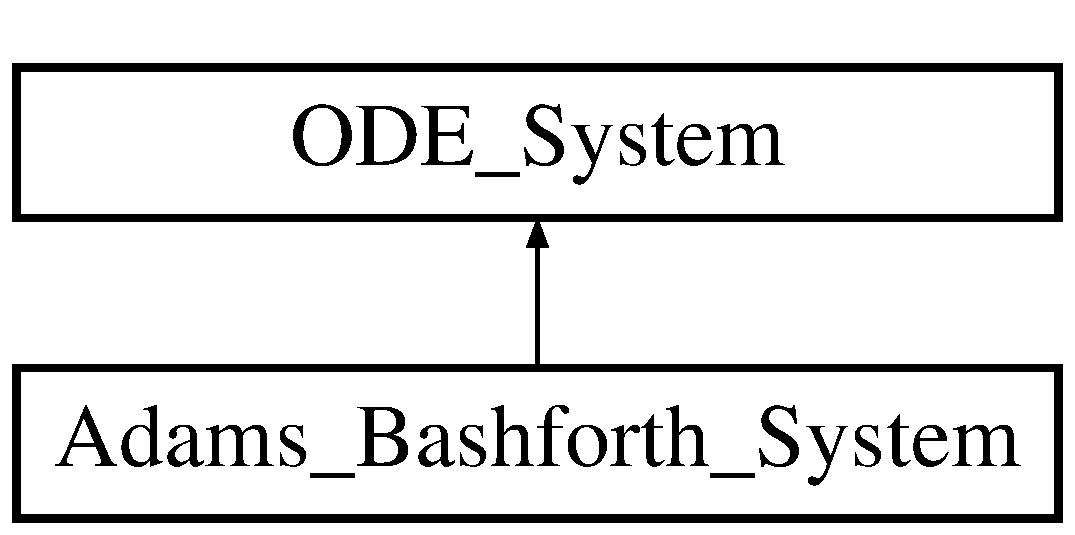
\includegraphics[height=2.000000cm]{class_adams___bashforth___system}
\end{center}
\end{figure}
\subsection*{Public Member Functions}
\begin{DoxyCompactItemize}
\item 
\mbox{\Hypertarget{class_adams___bashforth___system_a6fabff52bfd4dee448d918ac40efb1ef}\label{class_adams___bashforth___system_a6fabff52bfd4dee448d918ac40efb1ef}} 
\mbox{\hyperlink{class_adams___bashforth___system_a6fabff52bfd4dee448d918ac40efb1ef}{Adams\+\_\+\+Bashforth\+\_\+\+System}} (Real \mbox{\hyperlink{class_o_d_e___system_a1947b357608babc98c5e79d645e24c3c}{t0}}, Real \mbox{\hyperlink{class_o_d_e___system_a5c5a0dd9f04dfb8d8a84d49b741773af}{tn}}, const Vector \&\mbox{\hyperlink{class_o_d_e___system_a1379137a4480e5861fd1911bc061f908}{y00}}, const Matrix \&\mbox{\hyperlink{class_o_d_e___system_a632009677e80b62a1996e842398bf8b6}{A}}, Vector \mbox{\hyperlink{class_o_d_e___system_a5a294fda765e6cbfd7dfda43755d2c55}{g}}(Real), int \mbox{\hyperlink{class_adams___bashforth___system_abc285f795f629737fb82c223b896c5e8}{step}}, int \mbox{\hyperlink{class_o_d_e___system_a46e5ee402ffc7c500dccad753a1fba36}{M}})
\begin{DoxyCompactList}\small\item\em Constructor. Initialize data sturcture. \end{DoxyCompactList}\item 
\mbox{\Hypertarget{class_adams___bashforth___system_af183f3376f969b50d1a09305a5bff62b}\label{class_adams___bashforth___system_af183f3376f969b50d1a09305a5bff62b}} 
\mbox{\hyperlink{class_adams___bashforth___system_af183f3376f969b50d1a09305a5bff62b}{$\sim$\+Adams\+\_\+\+Bashforth\+\_\+\+System}} () override
\begin{DoxyCompactList}\small\item\em Destructor. Deallocate memory used by std\+::vector objects. \end{DoxyCompactList}\item 
void \mbox{\hyperlink{class_adams___bashforth___system_aa34bb9a1367a3b15f606ff49054e9ece}{solve}} () override
\begin{DoxyCompactList}\small\item\em Implement Adams Bashforth method and store the solution at all time steps in the attribute solution. \end{DoxyCompactList}\end{DoxyCompactItemize}
\subsection*{Protected Attributes}
\begin{DoxyCompactItemize}
\item 
\mbox{\Hypertarget{class_adams___bashforth___system_abc285f795f629737fb82c223b896c5e8}\label{class_adams___bashforth___system_abc285f795f629737fb82c223b896c5e8}} 
int \mbox{\hyperlink{class_adams___bashforth___system_abc285f795f629737fb82c223b896c5e8}{step}}
\begin{DoxyCompactList}\small\item\em step order of the method \end{DoxyCompactList}\end{DoxyCompactItemize}


\subsection{Detailed Description}
Inheritance of class \mbox{\hyperlink{class_o_d_e___system}{O\+D\+E\+\_\+\+System}}\+: Solving the vectorial system by means of Adams Bashforth method. 

\subsection{Member Function Documentation}
\mbox{\Hypertarget{class_adams___bashforth___system_aa34bb9a1367a3b15f606ff49054e9ece}\label{class_adams___bashforth___system_aa34bb9a1367a3b15f606ff49054e9ece}} 
\index{Adams\+\_\+\+Bashforth\+\_\+\+System@{Adams\+\_\+\+Bashforth\+\_\+\+System}!solve@{solve}}
\index{solve@{solve}!Adams\+\_\+\+Bashforth\+\_\+\+System@{Adams\+\_\+\+Bashforth\+\_\+\+System}}
\subsubsection{\texorpdfstring{solve()}{solve()}}
{\footnotesize\ttfamily void Adams\+\_\+\+Bashforth\+\_\+\+System\+::solve (\begin{DoxyParamCaption}{ }\end{DoxyParamCaption})\hspace{0.3cm}{\ttfamily [override]}, {\ttfamily [virtual]}}



Implement Adams Bashforth method and store the solution at all time steps in the attribute solution. 

f(t,y)=A$\ast$y+g(t)~\newline
step=1\+: Adams Bashforth method is the same as Forward Euler method. ~\newline
step=2\+: y\+\_\+\{n+2\}=y\+\_\+\{n+1\}+h$\ast$(3/2$\ast$f(t\+\_\+\{n+1\},y\+\_\+\{n+1\})-\/1/2$\ast$f(t\+\_\+n,y\+\_\+n)) ~\newline
step=3\+: y\+\_\+\{n+3\}=y\+\_\+\{n+2\}+h$\ast$(23/12$\ast$f(t\+\_\+\{n+2\},y\+\_\+\{n+2\})-\/16/12$\ast$f(t\+\_\+\{n+1\},y\+\_\+\{n+1\})+5/12$\ast$f(t\+\_\+n,y\+\_\+n))~\newline
step=4\+: y\+\_\+\{n+4\}=y\+\_\+\{n+3\}+h$\ast$(55/24$\ast$f(t\+\_\+\{n+3\},y\+\_\+\{n+3\})-\/59/24$\ast$f(t\+\_\+\{n+2\},y\+\_\+\{n+2\})+37/24$\ast$f(t\+\_\+\{n+1\},y\+\_\+\{n+1\})-\/9/24$\ast$f(t\+\_\+n,y\+\_\+n)) ~\newline


Implements \mbox{\hyperlink{class_o_d_e___system_a78a058382148b745fa458f0b9f52f47c}{O\+D\+E\+\_\+\+System}}.



The documentation for this class was generated from the following files\+:\begin{DoxyCompactItemize}
\item 
/\+Users/jiahuawu/\+Desktop/\+O\+D\+E\+\_\+\+Solver2/O\+D\+E\+\_\+system.\+h\item 
/\+Users/jiahuawu/\+Desktop/\+O\+D\+E\+\_\+\+Solver2/O\+D\+E\+\_\+system.\+cpp\end{DoxyCompactItemize}

\hypertarget{class_data___reader}{}\section{Data\+\_\+\+Reader Class Reference}
\label{class_data___reader}\index{Data\+\_\+\+Reader@{Data\+\_\+\+Reader}}


Inheritance of class \mbox{\hyperlink{class_reader}{Reader}} which specializes in reading data from files.  




{\ttfamily \#include $<$input.\+h$>$}

Inheritance diagram for Data\+\_\+\+Reader\+:\begin{figure}[H]
\begin{center}
\leavevmode
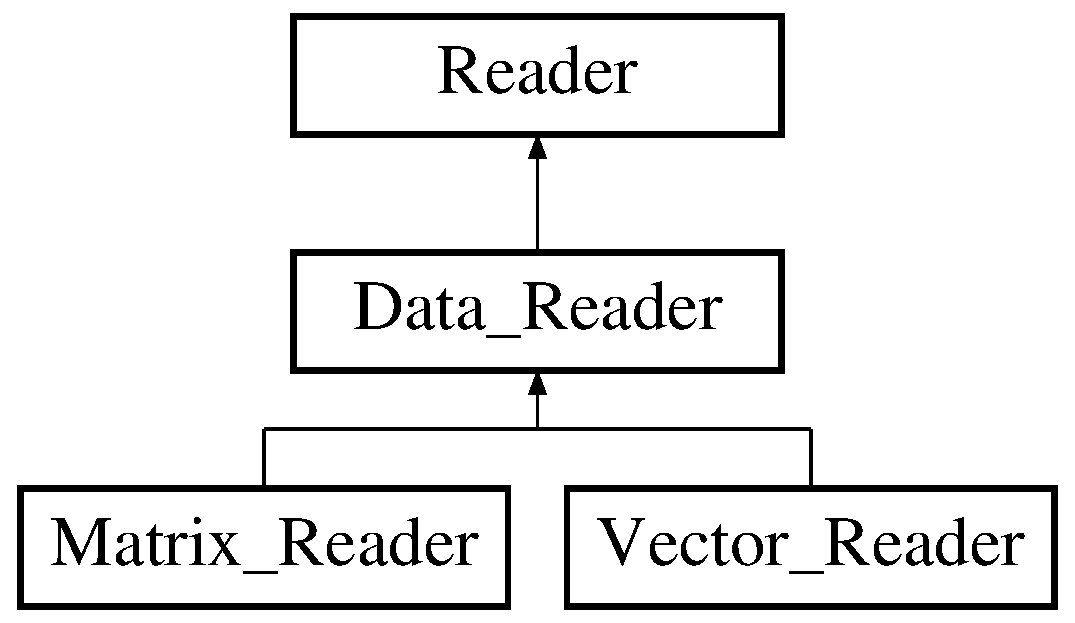
\includegraphics[height=3.000000cm]{class_data___reader}
\end{center}
\end{figure}
\subsection*{Public Member Functions}
\begin{DoxyCompactItemize}
\item 
\mbox{\Hypertarget{class_data___reader_a8ea116155d708b4516786730fdeb93bb}\label{class_data___reader_a8ea116155d708b4516786730fdeb93bb}} 
\mbox{\hyperlink{class_data___reader_a8ea116155d708b4516786730fdeb93bb}{Data\+\_\+\+Reader}} (const string \&\mbox{\hyperlink{class_reader_a4f3eaccb117f248d4649ffb4e793a23d}{path}}, char \mbox{\hyperlink{class_data___reader_ac05700473d754089d7f30d2cc7dccce9}{delimiter}})
\begin{DoxyCompactList}\small\item\em Constructor. Initialize the attributes with the input path and delimiter. \end{DoxyCompactList}\item 
\mbox{\Hypertarget{class_data___reader_a2c1fa3b33d6bc8aab051878e1d3395cf}\label{class_data___reader_a2c1fa3b33d6bc8aab051878e1d3395cf}} 
virtual \mbox{\hyperlink{class_data___reader_a2c1fa3b33d6bc8aab051878e1d3395cf}{$\sim$\+Data\+\_\+\+Reader}} ()=default
\begin{DoxyCompactList}\small\item\em Default destructor to be override. \end{DoxyCompactList}\end{DoxyCompactItemize}
\subsection*{Protected Attributes}
\begin{DoxyCompactItemize}
\item 
\mbox{\Hypertarget{class_data___reader_ac05700473d754089d7f30d2cc7dccce9}\label{class_data___reader_ac05700473d754089d7f30d2cc7dccce9}} 
char \mbox{\hyperlink{class_data___reader_ac05700473d754089d7f30d2cc7dccce9}{delimiter}}
\begin{DoxyCompactList}\small\item\em delimiter used in the file to be read \end{DoxyCompactList}\end{DoxyCompactItemize}


\subsection{Detailed Description}
Inheritance of class \mbox{\hyperlink{class_reader}{Reader}} which specializes in reading data from files. 

The documentation for this class was generated from the following files\+:\begin{DoxyCompactItemize}
\item 
/\+Users/jiahuawu/\+Desktop/\+O\+D\+E\+\_\+\+Solver2/input.\+h\item 
/\+Users/jiahuawu/\+Desktop/\+O\+D\+E\+\_\+\+Solver2/input.\+cpp\end{DoxyCompactItemize}

\hypertarget{classdimnotmatch}{}\section{dimnotmatch Class Reference}
\label{classdimnotmatch}\index{dimnotmatch@{dimnotmatch}}


Inheritance of class exception\+: deal with dimension incompatible problem.  




{\ttfamily \#include $<$O\+D\+E\+\_\+solver.\+h$>$}

Inheritance diagram for dimnotmatch\+:\begin{figure}[H]
\begin{center}
\leavevmode
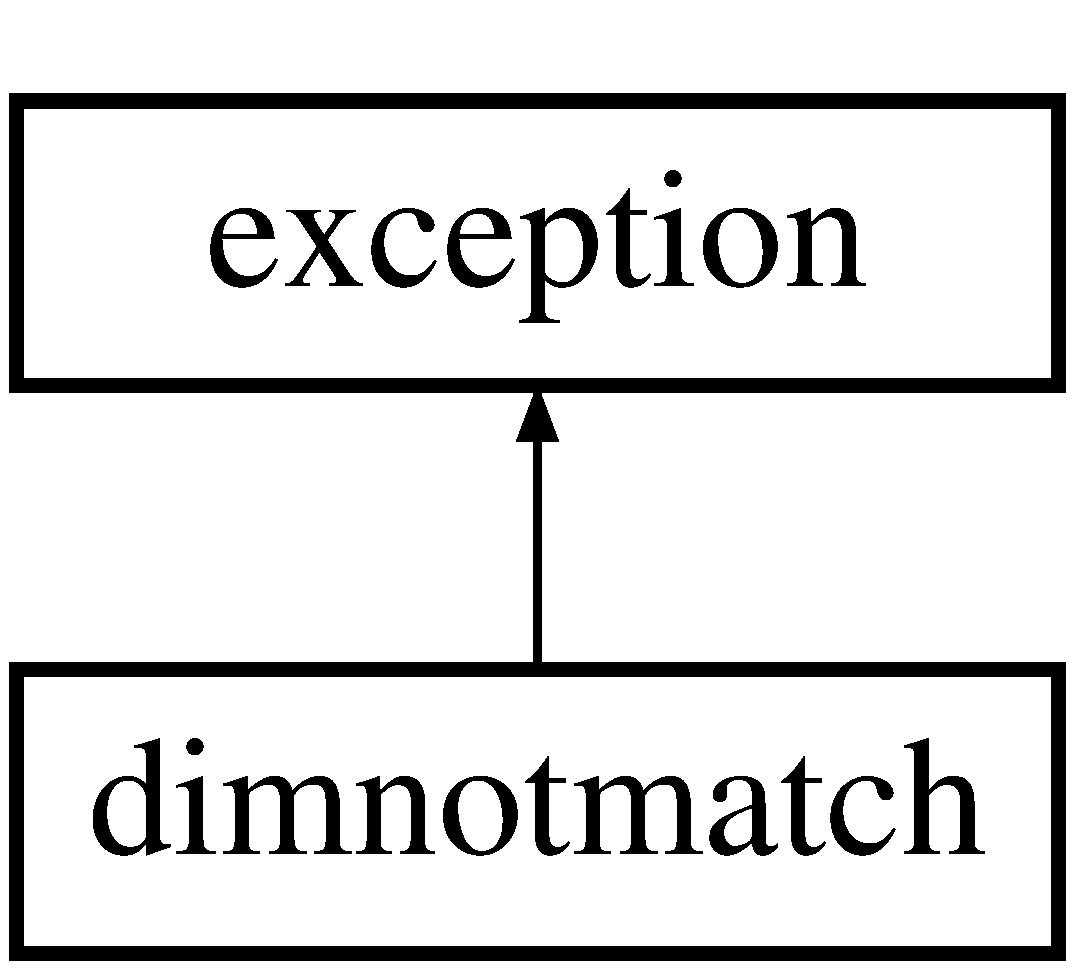
\includegraphics[height=2.000000cm]{classdimnotmatch}
\end{center}
\end{figure}
\subsection*{Public Member Functions}
\begin{DoxyCompactItemize}
\item 
\mbox{\Hypertarget{classdimnotmatch_af8ab958cff29859339d5493960a0c444}\label{classdimnotmatch_af8ab958cff29859339d5493960a0c444}} 
virtual const char $\ast$ {\bfseries what} () const  throw ()
\end{DoxyCompactItemize}


\subsection{Detailed Description}
Inheritance of class exception\+: deal with dimension incompatible problem. 

The documentation for this class was generated from the following file\+:\begin{DoxyCompactItemize}
\item 
/\+Users/jiahuawu/\+Desktop/\+O\+D\+E\+\_\+\+Solver/O\+D\+E\+\_\+solver.\+h\end{DoxyCompactItemize}

\hypertarget{class_forward_euler___system}{}\section{Forward\+Euler\+\_\+\+System Class Reference}
\label{class_forward_euler___system}\index{Forward\+Euler\+\_\+\+System@{Forward\+Euler\+\_\+\+System}}


Inheritance of class \mbox{\hyperlink{class_o_d_e___system}{O\+D\+E\+\_\+\+System}}\+: Solving the vectorial system by means of forward Euler method.  




{\ttfamily \#include $<$O\+D\+E\+\_\+\+System.\+h$>$}

Inheritance diagram for Forward\+Euler\+\_\+\+System\+:\begin{figure}[H]
\begin{center}
\leavevmode
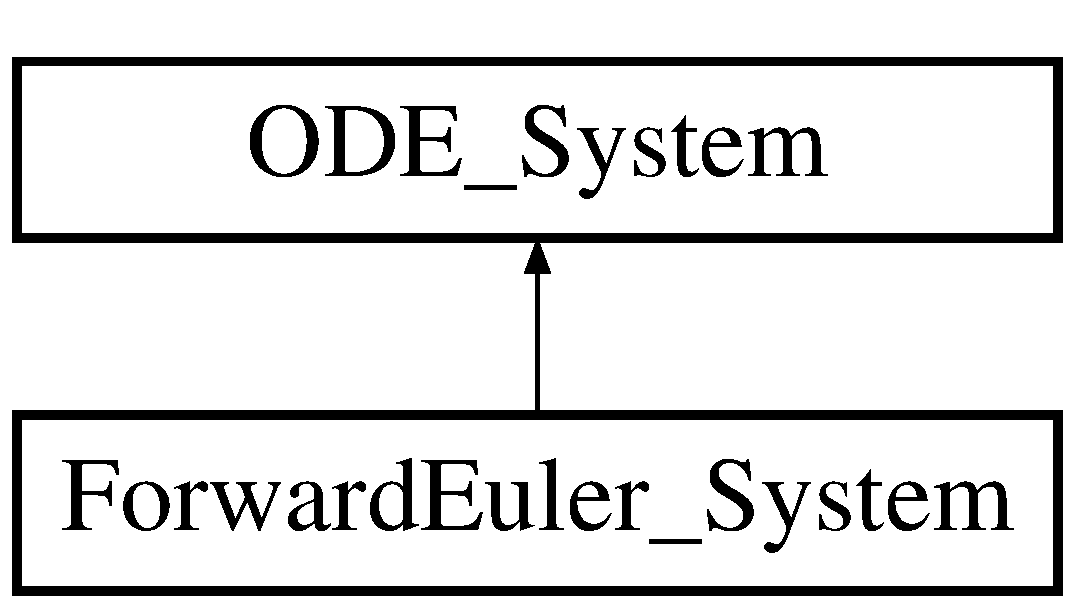
\includegraphics[height=2.000000cm]{class_forward_euler___system}
\end{center}
\end{figure}
\subsection*{Public Member Functions}
\begin{DoxyCompactItemize}
\item 
\mbox{\Hypertarget{class_forward_euler___system_a346bc0f2ebda791edd4cea34761cc7f7}\label{class_forward_euler___system_a346bc0f2ebda791edd4cea34761cc7f7}} 
\mbox{\hyperlink{class_forward_euler___system_a346bc0f2ebda791edd4cea34761cc7f7}{Forward\+Euler\+\_\+\+System}} (double \mbox{\hyperlink{class_o_d_e___system_a1947b357608babc98c5e79d645e24c3c}{t0}}, double \mbox{\hyperlink{class_o_d_e___system_a5c5a0dd9f04dfb8d8a84d49b741773af}{tn}}, const Vector \&\mbox{\hyperlink{class_o_d_e___system_a1379137a4480e5861fd1911bc061f908}{y00}}, const Matrix \&\mbox{\hyperlink{class_o_d_e___system_a632009677e80b62a1996e842398bf8b6}{A}}, Vector \mbox{\hyperlink{class_o_d_e___system_a2dee2a4b3468547c3ddab15edfc8ddfd}{g}}(Real))
\begin{DoxyCompactList}\small\item\em Constructor. Initialize data sturcture. \end{DoxyCompactList}\item 
\mbox{\Hypertarget{class_forward_euler___system_a97a3dd10d62f962b537ac616e84463a5}\label{class_forward_euler___system_a97a3dd10d62f962b537ac616e84463a5}} 
\mbox{\hyperlink{class_forward_euler___system_a97a3dd10d62f962b537ac616e84463a5}{$\sim$\+Forward\+Euler\+\_\+\+System}} () override
\begin{DoxyCompactList}\small\item\em Destructor. Deallocate memory used by std\+::vector objects. \end{DoxyCompactList}\item 
void \mbox{\hyperlink{class_forward_euler___system_a52532a83a016d8478a7c458881b214b4}{solve}} (int M) override
\begin{DoxyCompactList}\small\item\em Implement explicit forward euler method and store the solution at all time steps in the attribute solution. \end{DoxyCompactList}\end{DoxyCompactItemize}
\subsection*{Additional Inherited Members}


\subsection{Detailed Description}
Inheritance of class \mbox{\hyperlink{class_o_d_e___system}{O\+D\+E\+\_\+\+System}}\+: Solving the vectorial system by means of forward Euler method. 

\subsection{Member Function Documentation}
\mbox{\Hypertarget{class_forward_euler___system_a52532a83a016d8478a7c458881b214b4}\label{class_forward_euler___system_a52532a83a016d8478a7c458881b214b4}} 
\index{Forward\+Euler\+\_\+\+System@{Forward\+Euler\+\_\+\+System}!solve@{solve}}
\index{solve@{solve}!Forward\+Euler\+\_\+\+System@{Forward\+Euler\+\_\+\+System}}
\subsubsection{\texorpdfstring{solve()}{solve()}}
{\footnotesize\ttfamily void Forward\+Euler\+\_\+\+System\+::solve (\begin{DoxyParamCaption}\item[{int}]{M }\end{DoxyParamCaption})\hspace{0.3cm}{\ttfamily [override]}, {\ttfamily [virtual]}}



Implement explicit forward euler method and store the solution at all time steps in the attribute solution. 

f(t,y)=A$\ast$y+g(t)~\newline
y\+\_\+\{n+1\}=y\+\_\+n+f(t\+\_\+n,y\+\_\+n)$\ast$h ~\newline

\begin{DoxyParams}{Parameters}
{\em M} & number of time steps \\
\hline
\end{DoxyParams}


Implements \mbox{\hyperlink{class_o_d_e___system_a5fe78282ecf67d851f1a2363a028e6dd}{O\+D\+E\+\_\+\+System}}.



The documentation for this class was generated from the following files\+:\begin{DoxyCompactItemize}
\item 
/\+Users/jiahuawu/\+Desktop/\+O\+D\+E\+\_\+\+Solver/O\+D\+E\+\_\+\+System.\+h\item 
/\+Users/jiahuawu/\+Desktop/\+O\+D\+E\+\_\+\+Solver/O\+D\+E\+\_\+\+System.\+cpp\end{DoxyCompactItemize}

\hypertarget{classfunction__reader}{}\section{function\+\_\+reader Class Reference}
\label{classfunction__reader}\index{function\+\_\+reader@{function\+\_\+reader}}
Inheritance diagram for function\+\_\+reader\+:\begin{figure}[H]
\begin{center}
\leavevmode
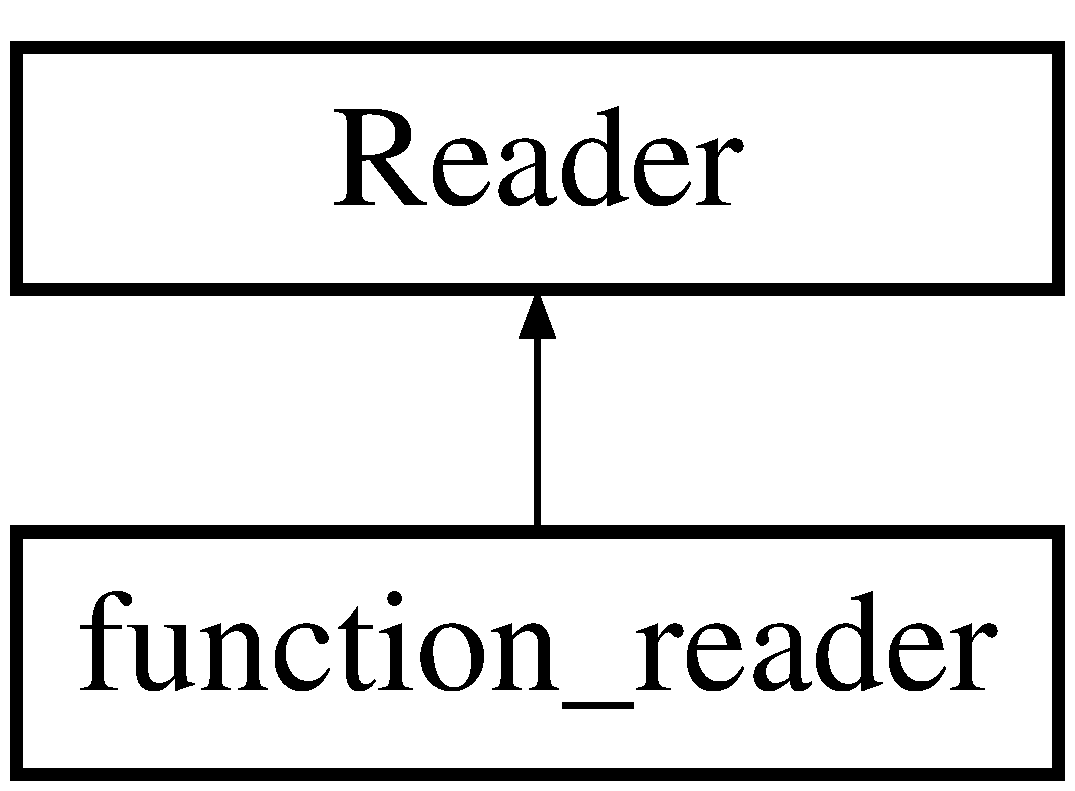
\includegraphics[height=2.000000cm]{classfunction__reader}
\end{center}
\end{figure}
\subsection*{Additional Inherited Members}


The documentation for this class was generated from the following file\+:\begin{DoxyCompactItemize}
\item 
/\+Users/jiahuawu/\+Desktop/\+O\+D\+E\+\_\+\+Solver/include/Input.\+h\end{DoxyCompactItemize}

\hypertarget{class_matrix___reader}{}\section{Matrix\+\_\+\+Reader Class Reference}
\label{class_matrix___reader}\index{Matrix\+\_\+\+Reader@{Matrix\+\_\+\+Reader}}


Inheritance of class \mbox{\hyperlink{class_data___reader}{Data\+\_\+\+Reader}} which specializes in reading files storing a matrix.  




{\ttfamily \#include $<$input.\+h$>$}

Inheritance diagram for Matrix\+\_\+\+Reader\+:\begin{figure}[H]
\begin{center}
\leavevmode
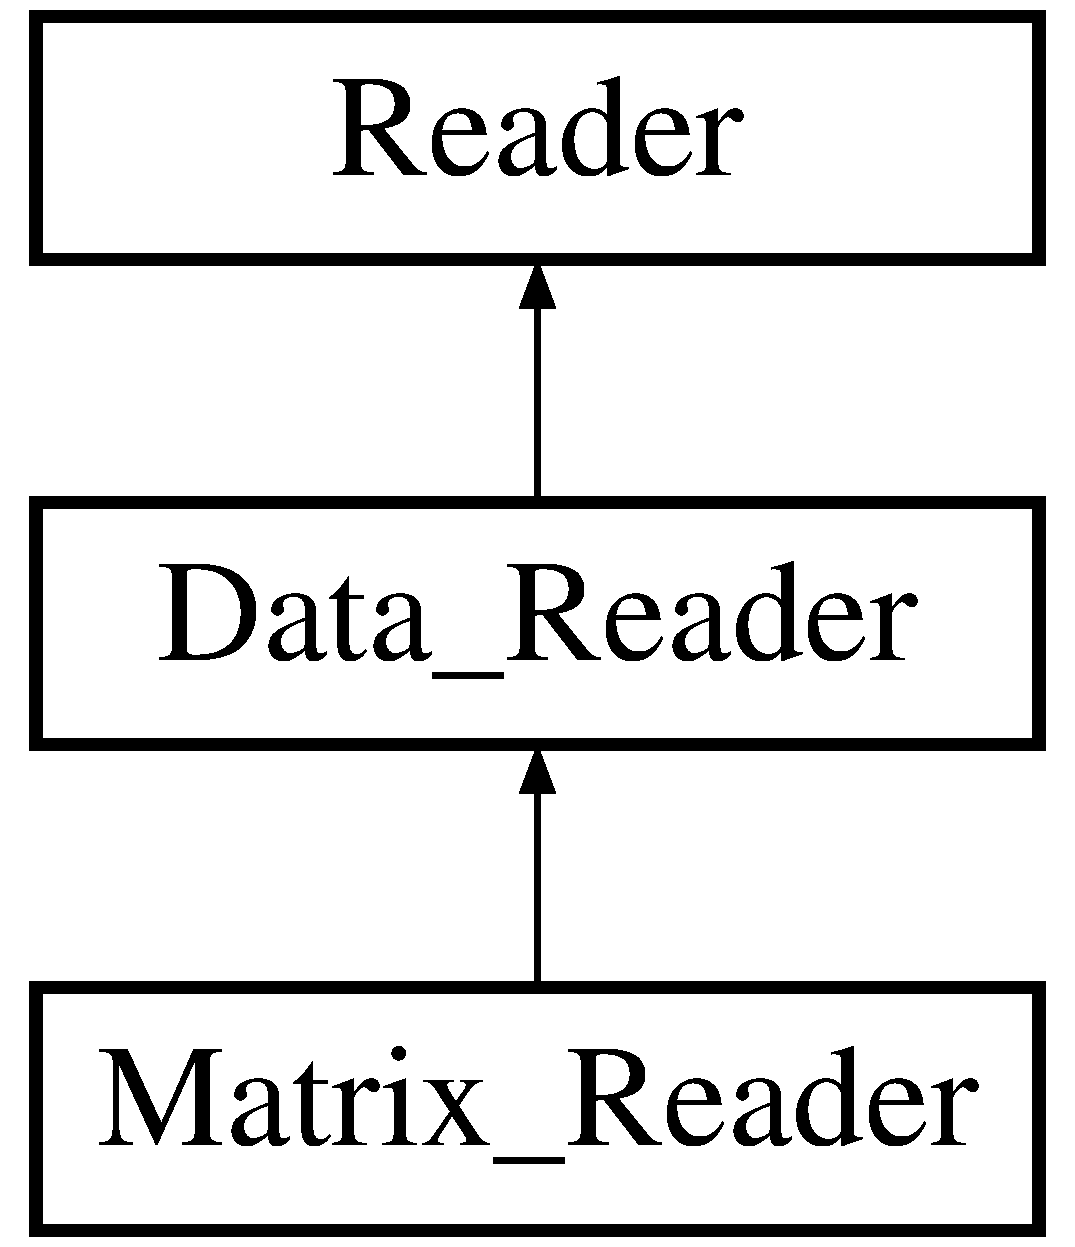
\includegraphics[height=3.000000cm]{class_matrix___reader}
\end{center}
\end{figure}
\subsection*{Public Member Functions}
\begin{DoxyCompactItemize}
\item 
\mbox{\Hypertarget{class_matrix___reader_aead34cd16f7ef3c2cbeffa390283d909}\label{class_matrix___reader_aead34cd16f7ef3c2cbeffa390283d909}} 
\mbox{\hyperlink{class_matrix___reader_aead34cd16f7ef3c2cbeffa390283d909}{Matrix\+\_\+\+Reader}} (const string \&\mbox{\hyperlink{class_reader_a4f3eaccb117f248d4649ffb4e793a23d}{path}}, char \mbox{\hyperlink{class_data___reader_ac05700473d754089d7f30d2cc7dccce9}{delimiter}}=\textquotesingle{} \textquotesingle{})
\begin{DoxyCompactList}\small\item\em Constructor. Initialize data structure with the input arguments. \end{DoxyCompactList}\item 
\mbox{\Hypertarget{class_matrix___reader_a576e866dc168437fd9272a0331b0a946}\label{class_matrix___reader_a576e866dc168437fd9272a0331b0a946}} 
\mbox{\hyperlink{class_matrix___reader_a576e866dc168437fd9272a0331b0a946}{$\sim$\+Matrix\+\_\+\+Reader}} () override
\begin{DoxyCompactList}\small\item\em Destructor. Deallocate the memory used by the Matrix attribute. \end{DoxyCompactList}\item 
\mbox{\Hypertarget{class_matrix___reader_a4543c9a568c9a14e141c9f2606b6ae0d}\label{class_matrix___reader_a4543c9a568c9a14e141c9f2606b6ae0d}} 
Matrix \mbox{\hyperlink{class_matrix___reader_a4543c9a568c9a14e141c9f2606b6ae0d}{access\+\_\+matrix}} () const
\begin{DoxyCompactList}\small\item\em Accessor. Access the matrix read from the file. \end{DoxyCompactList}\item 
\mbox{\Hypertarget{class_matrix___reader_a2476159bd0e9985f7e5059410199e56a}\label{class_matrix___reader_a2476159bd0e9985f7e5059410199e56a}} 
void \mbox{\hyperlink{class_matrix___reader_a2476159bd0e9985f7e5059410199e56a}{read\+\_\+in}} () override
\begin{DoxyCompactList}\small\item\em Read the file from the path attribute and assign it to the matrix attribute. \end{DoxyCompactList}\end{DoxyCompactItemize}
\subsection*{Protected Attributes}
\begin{DoxyCompactItemize}
\item 
\mbox{\Hypertarget{class_matrix___reader_a4a8f9b95e6361b1a58a53a3e54c0b0bb}\label{class_matrix___reader_a4a8f9b95e6361b1a58a53a3e54c0b0bb}} 
Matrix \mbox{\hyperlink{class_matrix___reader_a4a8f9b95e6361b1a58a53a3e54c0b0bb}{A}}
\begin{DoxyCompactList}\small\item\em Matrix read from the file. \end{DoxyCompactList}\end{DoxyCompactItemize}


\subsection{Detailed Description}
Inheritance of class \mbox{\hyperlink{class_data___reader}{Data\+\_\+\+Reader}} which specializes in reading files storing a matrix. 

The documentation for this class was generated from the following files\+:\begin{DoxyCompactItemize}
\item 
/\+Users/jiahuawu/\+Desktop/\+O\+D\+E\+\_\+\+Solver2/input.\+h\item 
/\+Users/jiahuawu/\+Desktop/\+O\+D\+E\+\_\+\+Solver2/input.\+cpp\end{DoxyCompactItemize}

\hypertarget{class_o_d_e___system}{}\section{O\+D\+E\+\_\+\+System Class Reference}
\label{class_o_d_e___system}\index{O\+D\+E\+\_\+\+System@{O\+D\+E\+\_\+\+System}}


{\ttfamily \#include $<$O\+D\+E\+\_\+\+System.\+h$>$}

Inheritance diagram for O\+D\+E\+\_\+\+System\+:\begin{figure}[H]
\begin{center}
\leavevmode
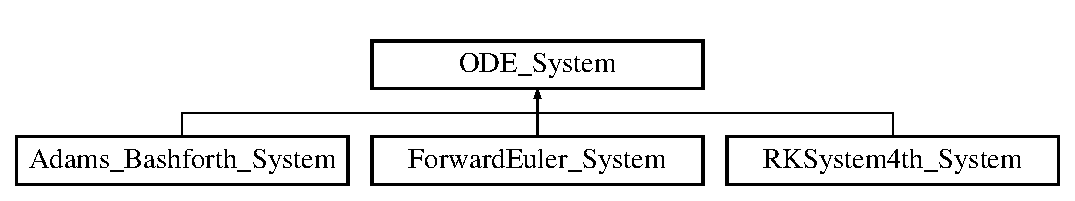
\includegraphics[height=2.000000cm]{class_o_d_e___system}
\end{center}
\end{figure}
\subsection*{Public Types}
\begin{DoxyCompactItemize}
\item 
\mbox{\Hypertarget{class_o_d_e___system_a9ff6775dafbba78d49f164174aa7074e}\label{class_o_d_e___system_a9ff6775dafbba78d49f164174aa7074e}} 
typedef Vector($\ast$ \mbox{\hyperlink{class_o_d_e___system_a9ff6775dafbba78d49f164174aa7074e}{Funpointer}}) (Real)
\begin{DoxyCompactList}\small\item\em Define the function pointer type. \end{DoxyCompactList}\end{DoxyCompactItemize}
\subsection*{Public Member Functions}
\begin{DoxyCompactItemize}
\item 
\mbox{\Hypertarget{class_o_d_e___system_a39f84fa09d28b6ecf4de1e57b480a568}\label{class_o_d_e___system_a39f84fa09d28b6ecf4de1e57b480a568}} 
\mbox{\hyperlink{class_o_d_e___system_a39f84fa09d28b6ecf4de1e57b480a568}{O\+D\+E\+\_\+\+System}} (double \mbox{\hyperlink{class_o_d_e___system_a1947b357608babc98c5e79d645e24c3c}{t0}}, double \mbox{\hyperlink{class_o_d_e___system_a5c5a0dd9f04dfb8d8a84d49b741773af}{tn}}, const Vector \&\mbox{\hyperlink{class_o_d_e___system_a1379137a4480e5861fd1911bc061f908}{y00}}, const Matrix \&\mbox{\hyperlink{class_o_d_e___system_a632009677e80b62a1996e842398bf8b6}{A}}, Vector \mbox{\hyperlink{class_o_d_e___system_a2dee2a4b3468547c3ddab15edfc8ddfd}{g}}(Real))
\begin{DoxyCompactList}\small\item\em Constructor. Initializes \mbox{\hyperlink{class_o_d_e___system}{O\+D\+E\+\_\+\+System}} data structures. \end{DoxyCompactList}\item 
\mbox{\Hypertarget{class_o_d_e___system_a1d38890ff0950344d4d34b9fab6a956b}\label{class_o_d_e___system_a1d38890ff0950344d4d34b9fab6a956b}} 
virtual \mbox{\hyperlink{class_o_d_e___system_a1d38890ff0950344d4d34b9fab6a956b}{$\sim$\+O\+D\+E\+\_\+\+System}} ()
\begin{DoxyCompactList}\small\item\em Destructor. Deallocate memory used by std\+::vector objects. \end{DoxyCompactList}\item 
\mbox{\Hypertarget{class_o_d_e___system_aebb5a7971ef1c429077155eec549f713}\label{class_o_d_e___system_aebb5a7971ef1c429077155eec549f713}} 
Matrix \mbox{\hyperlink{class_o_d_e___system_aebb5a7971ef1c429077155eec549f713}{access\+\_\+solution}} () const
\begin{DoxyCompactList}\small\item\em Accessor to get the solution. \end{DoxyCompactList}\item 
\mbox{\Hypertarget{class_o_d_e___system_a24094974423d600f580455427141fa3e}\label{class_o_d_e___system_a24094974423d600f580455427141fa3e}} 
void \mbox{\hyperlink{class_o_d_e___system_a24094974423d600f580455427141fa3e}{set\+\_\+A}} (const Matrix \&\mbox{\hyperlink{class_o_d_e___system_a632009677e80b62a1996e842398bf8b6}{A}})
\begin{DoxyCompactList}\small\item\em Set the Matrix A. \end{DoxyCompactList}\item 
\mbox{\Hypertarget{class_o_d_e___system_a6906f9069496452cab2b56b6a49635d1}\label{class_o_d_e___system_a6906f9069496452cab2b56b6a49635d1}} 
void \mbox{\hyperlink{class_o_d_e___system_a6906f9069496452cab2b56b6a49635d1}{set\+\_\+g}} (Vector \mbox{\hyperlink{class_o_d_e___system_a2dee2a4b3468547c3ddab15edfc8ddfd}{g}}(Real))
\begin{DoxyCompactList}\small\item\em Set the function g. \end{DoxyCompactList}\item 
\mbox{\Hypertarget{class_o_d_e___system_a1856c9b15a41ca733e509e44f4535f5f}\label{class_o_d_e___system_a1856c9b15a41ca733e509e44f4535f5f}} 
void \mbox{\hyperlink{class_o_d_e___system_a1856c9b15a41ca733e509e44f4535f5f}{set\+\_\+y0}} (const Vector \&y0)
\begin{DoxyCompactList}\small\item\em Set initial condition. \end{DoxyCompactList}\item 
virtual void \mbox{\hyperlink{class_o_d_e___system_a5fe78282ecf67d851f1a2363a028e6dd}{solve}} (int M)=0
\begin{DoxyCompactList}\small\item\em Pure virtual method. Call the solvers to solve the system. \end{DoxyCompactList}\item 
void \mbox{\hyperlink{class_o_d_e___system_ad07810b15fa1d891b64a83812433fef6}{write\+\_\+solution}} (string filename, int precision=5)
\begin{DoxyCompactList}\small\item\em Output the solution as filetype given by the user~\newline
. \end{DoxyCompactList}\end{DoxyCompactItemize}
\subsection*{Protected Attributes}
\begin{DoxyCompactItemize}
\item 
\mbox{\Hypertarget{class_o_d_e___system_a1947b357608babc98c5e79d645e24c3c}\label{class_o_d_e___system_a1947b357608babc98c5e79d645e24c3c}} 
Real \mbox{\hyperlink{class_o_d_e___system_a1947b357608babc98c5e79d645e24c3c}{t0}}
\begin{DoxyCompactList}\small\item\em Initial time. \end{DoxyCompactList}\item 
\mbox{\Hypertarget{class_o_d_e___system_a5c5a0dd9f04dfb8d8a84d49b741773af}\label{class_o_d_e___system_a5c5a0dd9f04dfb8d8a84d49b741773af}} 
Real \mbox{\hyperlink{class_o_d_e___system_a5c5a0dd9f04dfb8d8a84d49b741773af}{tn}}
\begin{DoxyCompactList}\small\item\em End time. \end{DoxyCompactList}\item 
\mbox{\Hypertarget{class_o_d_e___system_a1379137a4480e5861fd1911bc061f908}\label{class_o_d_e___system_a1379137a4480e5861fd1911bc061f908}} 
Vector \mbox{\hyperlink{class_o_d_e___system_a1379137a4480e5861fd1911bc061f908}{y00}}
\begin{DoxyCompactList}\small\item\em nitial condition \end{DoxyCompactList}\item 
\mbox{\Hypertarget{class_o_d_e___system_a2dee2a4b3468547c3ddab15edfc8ddfd}\label{class_o_d_e___system_a2dee2a4b3468547c3ddab15edfc8ddfd}} 
\mbox{\hyperlink{class_o_d_e___system_a9ff6775dafbba78d49f164174aa7074e}{Funpointer}} \mbox{\hyperlink{class_o_d_e___system_a2dee2a4b3468547c3ddab15edfc8ddfd}{g}}
\begin{DoxyCompactList}\small\item\em Function pointer storing the function g as defined in the problem. \end{DoxyCompactList}\item 
\mbox{\Hypertarget{class_o_d_e___system_a632009677e80b62a1996e842398bf8b6}\label{class_o_d_e___system_a632009677e80b62a1996e842398bf8b6}} 
Matrix \mbox{\hyperlink{class_o_d_e___system_a632009677e80b62a1996e842398bf8b6}{A}}
\begin{DoxyCompactList}\small\item\em Matrix A as defined in the problem. \end{DoxyCompactList}\item 
\mbox{\Hypertarget{class_o_d_e___system_ab2504680346a353e353f147f1ad9c51d}\label{class_o_d_e___system_ab2504680346a353e353f147f1ad9c51d}} 
Matrix \mbox{\hyperlink{class_o_d_e___system_ab2504680346a353e353f147f1ad9c51d}{solution}}
\begin{DoxyCompactList}\small\item\em Matrix storing the solution~\newline
ith row = solution vector at ith time step~\newline
jth col = solution of the jth component at all time steps. \end{DoxyCompactList}\end{DoxyCompactItemize}


\subsection{Detailed Description}
This abstract class stores essential ingredient of a vectorial ode system as well as a solution obtained by using specified solver functions. 

\subsection{Member Function Documentation}
\mbox{\Hypertarget{class_o_d_e___system_a5fe78282ecf67d851f1a2363a028e6dd}\label{class_o_d_e___system_a5fe78282ecf67d851f1a2363a028e6dd}} 
\index{O\+D\+E\+\_\+\+System@{O\+D\+E\+\_\+\+System}!solve@{solve}}
\index{solve@{solve}!O\+D\+E\+\_\+\+System@{O\+D\+E\+\_\+\+System}}
\subsubsection{\texorpdfstring{solve()}{solve()}}
{\footnotesize\ttfamily virtual void O\+D\+E\+\_\+\+System\+::solve (\begin{DoxyParamCaption}\item[{int}]{M }\end{DoxyParamCaption})\hspace{0.3cm}{\ttfamily [pure virtual]}}



Pure virtual method. Call the solvers to solve the system. 


\begin{DoxyParams}{Parameters}
{\em M} & number of time steps \\
\hline
\end{DoxyParams}


Implemented in \mbox{\hyperlink{class_r_k_system4th___system_ae36715c58bf1afc191394185f36eb611}{R\+K\+System4th\+\_\+\+System}}, \mbox{\hyperlink{class_adams___bashforth___system_acaf33d4f9f715a20a106f9029135cfe6}{Adams\+\_\+\+Bashforth\+\_\+\+System}}, and \mbox{\hyperlink{class_forward_euler___system_a52532a83a016d8478a7c458881b214b4}{Forward\+Euler\+\_\+\+System}}.

\mbox{\Hypertarget{class_o_d_e___system_ad07810b15fa1d891b64a83812433fef6}\label{class_o_d_e___system_ad07810b15fa1d891b64a83812433fef6}} 
\index{O\+D\+E\+\_\+\+System@{O\+D\+E\+\_\+\+System}!write\+\_\+solution@{write\+\_\+solution}}
\index{write\+\_\+solution@{write\+\_\+solution}!O\+D\+E\+\_\+\+System@{O\+D\+E\+\_\+\+System}}
\subsubsection{\texorpdfstring{write\+\_\+solution()}{write\_solution()}}
{\footnotesize\ttfamily void O\+D\+E\+\_\+\+System\+::write\+\_\+solution (\begin{DoxyParamCaption}\item[{string}]{filename,  }\item[{int}]{precision = {\ttfamily 5} }\end{DoxyParamCaption})}



Output the solution as filetype given by the user~\newline
. 


\begin{DoxyParams}{Parameters}
{\em precision} & number of significant numbers~\newline
\\
\hline
{\em filename} & name of the file in form of a string \\
\hline
\end{DoxyParams}


The documentation for this class was generated from the following files\+:\begin{DoxyCompactItemize}
\item 
/\+Users/jiahuawu/\+Desktop/\+O\+D\+E\+\_\+\+Solver/O\+D\+E\+\_\+\+System.\+h\item 
/\+Users/jiahuawu/\+Desktop/\+O\+D\+E\+\_\+\+Solver/O\+D\+E\+\_\+\+System.\+cpp\end{DoxyCompactItemize}

\hypertarget{classordernotmatch}{}\section{ordernotmatch Class Reference}
\label{classordernotmatch}\index{ordernotmatch@{ordernotmatch}}


Inheritance of class exception\+: we can only deal with Adams Bashforth method with order 1 2 3 4.  




{\ttfamily \#include $<$O\+D\+E\+\_\+solver.\+h$>$}

Inheritance diagram for ordernotmatch\+:\begin{figure}[H]
\begin{center}
\leavevmode
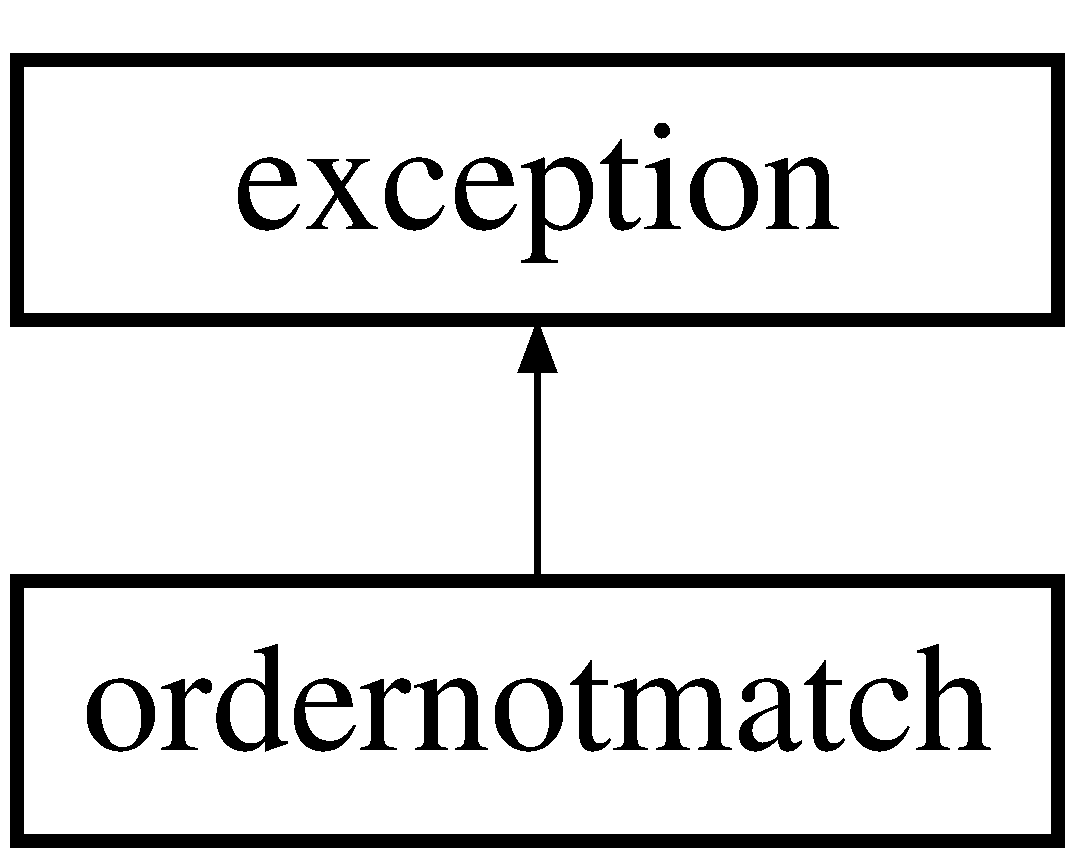
\includegraphics[height=2.000000cm]{classordernotmatch}
\end{center}
\end{figure}
\subsection*{Public Member Functions}
\begin{DoxyCompactItemize}
\item 
\mbox{\Hypertarget{classordernotmatch_a3cd5dc7766d282739bcaa67a544b42cb}\label{classordernotmatch_a3cd5dc7766d282739bcaa67a544b42cb}} 
virtual const char $\ast$ {\bfseries what} () const  throw ()
\end{DoxyCompactItemize}


\subsection{Detailed Description}
Inheritance of class exception\+: we can only deal with Adams Bashforth method with order 1 2 3 4. 

The documentation for this class was generated from the following file\+:\begin{DoxyCompactItemize}
\item 
/\+Users/jiahuawu/\+Desktop/\+O\+D\+E\+\_\+\+Solver2/O\+D\+E\+\_\+solver.\+h\end{DoxyCompactItemize}

\hypertarget{class_reader}{}\section{Reader Class Reference}
\label{class_reader}\index{Reader@{Reader}}


Abstract class of readers.  




{\ttfamily \#include $<$input.\+h$>$}

Inheritance diagram for Reader\+:\begin{figure}[H]
\begin{center}
\leavevmode
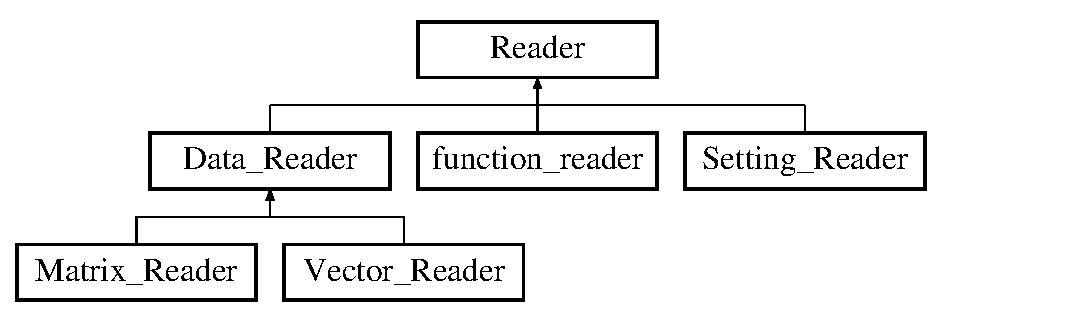
\includegraphics[height=3.000000cm]{class_reader}
\end{center}
\end{figure}
\subsection*{Public Member Functions}
\begin{DoxyCompactItemize}
\item 
\mbox{\Hypertarget{class_reader_a14282e3b34a1a2c8a8b2448a76edbf64}\label{class_reader_a14282e3b34a1a2c8a8b2448a76edbf64}} 
\mbox{\hyperlink{class_reader_a14282e3b34a1a2c8a8b2448a76edbf64}{Reader}} (const string \&\mbox{\hyperlink{class_reader_a4f3eaccb117f248d4649ffb4e793a23d}{path}})
\begin{DoxyCompactList}\small\item\em Constructor. Initialize the attribute path with the path given. \end{DoxyCompactList}\item 
\mbox{\Hypertarget{class_reader_ae95b8c18df56f806ca619f3d06326d63}\label{class_reader_ae95b8c18df56f806ca619f3d06326d63}} 
virtual void \mbox{\hyperlink{class_reader_ae95b8c18df56f806ca619f3d06326d63}{read\+\_\+in}} ()=0
\begin{DoxyCompactList}\small\item\em Pure virtual function for reading in from files. \end{DoxyCompactList}\end{DoxyCompactItemize}
\subsection*{Protected Attributes}
\begin{DoxyCompactItemize}
\item 
\mbox{\Hypertarget{class_reader_a4f3eaccb117f248d4649ffb4e793a23d}\label{class_reader_a4f3eaccb117f248d4649ffb4e793a23d}} 
string \mbox{\hyperlink{class_reader_a4f3eaccb117f248d4649ffb4e793a23d}{path}}
\begin{DoxyCompactList}\small\item\em Path of the file to be read. \end{DoxyCompactList}\end{DoxyCompactItemize}


\subsection{Detailed Description}
Abstract class of readers. 

The documentation for this class was generated from the following files\+:\begin{DoxyCompactItemize}
\item 
/\+Users/jiahuawu/\+Desktop/\+O\+D\+E\+\_\+\+Solver2/input.\+h\item 
/\+Users/jiahuawu/\+Desktop/\+O\+D\+E\+\_\+\+Solver2/input.\+cpp\end{DoxyCompactItemize}

\hypertarget{class_r_k_system4th___system}{}\section{R\+K\+System4th\+\_\+\+System Class Reference}
\label{class_r_k_system4th___system}\index{R\+K\+System4th\+\_\+\+System@{R\+K\+System4th\+\_\+\+System}}


Inheritance of class \mbox{\hyperlink{class_o_d_e___system}{O\+D\+E\+\_\+\+System}}\+: Solving the vectorial system by means of Runge Kutta 4th order method.  




{\ttfamily \#include $<$O\+D\+E\+\_\+system.\+h$>$}

Inheritance diagram for R\+K\+System4th\+\_\+\+System\+:\begin{figure}[H]
\begin{center}
\leavevmode
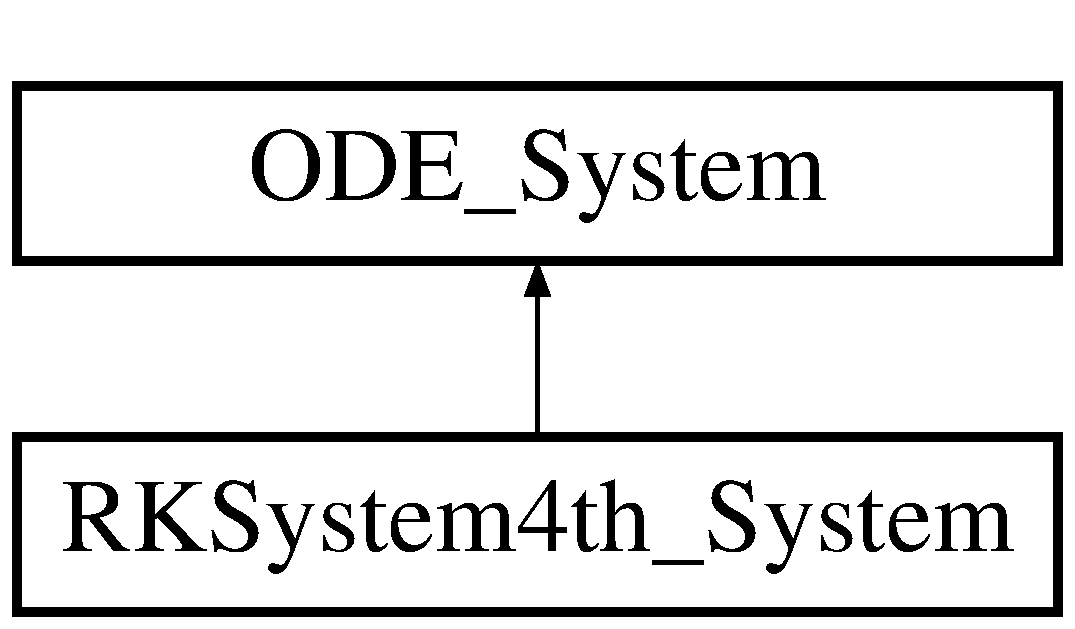
\includegraphics[height=2.000000cm]{class_r_k_system4th___system}
\end{center}
\end{figure}
\subsection*{Public Member Functions}
\begin{DoxyCompactItemize}
\item 
\mbox{\Hypertarget{class_r_k_system4th___system_a1c7317e4d0987ad09f2e58f931d8e5f0}\label{class_r_k_system4th___system_a1c7317e4d0987ad09f2e58f931d8e5f0}} 
\mbox{\hyperlink{class_r_k_system4th___system_a1c7317e4d0987ad09f2e58f931d8e5f0}{R\+K\+System4th\+\_\+\+System}} (Real \mbox{\hyperlink{class_o_d_e___system_a1947b357608babc98c5e79d645e24c3c}{t0}}, Real \mbox{\hyperlink{class_o_d_e___system_a5c5a0dd9f04dfb8d8a84d49b741773af}{tn}}, const Vector \&\mbox{\hyperlink{class_o_d_e___system_a1379137a4480e5861fd1911bc061f908}{y00}}, const Matrix \&\mbox{\hyperlink{class_o_d_e___system_a632009677e80b62a1996e842398bf8b6}{A}}, Vector \mbox{\hyperlink{class_o_d_e___system_a5a294fda765e6cbfd7dfda43755d2c55}{g}}(Real), int \mbox{\hyperlink{class_o_d_e___system_a46e5ee402ffc7c500dccad753a1fba36}{M}})
\begin{DoxyCompactList}\small\item\em Constructor. Initialize data sturcture. \end{DoxyCompactList}\item 
\mbox{\Hypertarget{class_r_k_system4th___system_aae823a4345fcf79cde38b100e473346f}\label{class_r_k_system4th___system_aae823a4345fcf79cde38b100e473346f}} 
\mbox{\hyperlink{class_r_k_system4th___system_aae823a4345fcf79cde38b100e473346f}{$\sim$\+R\+K\+System4th\+\_\+\+System}} () override
\begin{DoxyCompactList}\small\item\em Destructor. Deallocate memory used by std\+::vector objects. \end{DoxyCompactList}\item 
void \mbox{\hyperlink{class_r_k_system4th___system_ae7e9125546c6590f50d581f5e6668c82}{solve}} () override
\begin{DoxyCompactList}\small\item\em Implement Adams Bashforth method and store the solution at all time steps in the attribute solution. \end{DoxyCompactList}\end{DoxyCompactItemize}
\subsection*{Additional Inherited Members}


\subsection{Detailed Description}
Inheritance of class \mbox{\hyperlink{class_o_d_e___system}{O\+D\+E\+\_\+\+System}}\+: Solving the vectorial system by means of Runge Kutta 4th order method. 

\subsection{Member Function Documentation}
\mbox{\Hypertarget{class_r_k_system4th___system_ae7e9125546c6590f50d581f5e6668c82}\label{class_r_k_system4th___system_ae7e9125546c6590f50d581f5e6668c82}} 
\index{R\+K\+System4th\+\_\+\+System@{R\+K\+System4th\+\_\+\+System}!solve@{solve}}
\index{solve@{solve}!R\+K\+System4th\+\_\+\+System@{R\+K\+System4th\+\_\+\+System}}
\subsubsection{\texorpdfstring{solve()}{solve()}}
{\footnotesize\ttfamily void R\+K\+System4th\+\_\+\+System\+::solve (\begin{DoxyParamCaption}{ }\end{DoxyParamCaption})\hspace{0.3cm}{\ttfamily [override]}, {\ttfamily [virtual]}}



Implement Adams Bashforth method and store the solution at all time steps in the attribute solution. 

f(t,y)=A$\ast$y+g(t) ~\newline
k\+\_\+1=f(t\+\_\+n,y\+\_\+n)) ~\newline
k\+\_\+2=f(t\+\_\+n+0.5$\ast$h,y\+\_\+n+0.5$\ast$k\+\_\+1)) ~\newline
k\+\_\+3=f(t\+\_\+n+0.5$\ast$h,y\+\_\+n+0.5$\ast$k\+\_\+2)) ~\newline
k\+\_\+4=f(t\+\_\+n+h,y\+\_\+n+k\+\_\+3)) ~\newline
y\+\_\+\{n+1\}=1/6$\ast$k\+\_\+1+1/3$\ast$k\+\_\+2+1/3$\ast$k\+\_\+3+1/6$\ast$k\+\_\+4 ~\newline


Implements \mbox{\hyperlink{class_o_d_e___system_a78a058382148b745fa458f0b9f52f47c}{O\+D\+E\+\_\+\+System}}.



The documentation for this class was generated from the following files\+:\begin{DoxyCompactItemize}
\item 
/\+Users/jiahuawu/\+Desktop/\+O\+D\+E\+\_\+\+Solver2/O\+D\+E\+\_\+system.\+h\item 
/\+Users/jiahuawu/\+Desktop/\+O\+D\+E\+\_\+\+Solver2/O\+D\+E\+\_\+system.\+cpp\end{DoxyCompactItemize}

\hypertarget{struct_setting}{}\section{Setting Struct Reference}
\label{struct_setting}\index{Setting@{Setting}}


Structure storing parameters read from the setting file.  




{\ttfamily \#include $<$input.\+h$>$}

\subsection*{Public Attributes}
\begin{DoxyCompactItemize}
\item 
\mbox{\Hypertarget{struct_setting_a7d0cd8484c787085547a178a311239bd}\label{struct_setting_a7d0cd8484c787085547a178a311239bd}} 
int {\bfseries M}
\item 
\mbox{\Hypertarget{struct_setting_ab12392850916088ffc92d7eeccf84950}\label{struct_setting_ab12392850916088ffc92d7eeccf84950}} 
int {\bfseries precision} = 5
\item 
\mbox{\Hypertarget{struct_setting_aa4971ccaf90929605fc4f326e9f0b08a}\label{struct_setting_aa4971ccaf90929605fc4f326e9f0b08a}} 
int {\bfseries usual\+\_\+function} = 1
\item 
\mbox{\Hypertarget{struct_setting_a60b5d988c449e64b535813eeff85a55b}\label{struct_setting_a60b5d988c449e64b535813eeff85a55b}} 
Real {\bfseries t0}
\item 
\mbox{\Hypertarget{struct_setting_a18996fc4e88679942fc70d4379053d77}\label{struct_setting_a18996fc4e88679942fc70d4379053d77}} 
Real {\bfseries tn}
\item 
\mbox{\Hypertarget{struct_setting_a9f9d6c2e92d90956166bbe755200c3a5}\label{struct_setting_a9f9d6c2e92d90956166bbe755200c3a5}} 
string {\bfseries path\+\_\+y00}
\item 
\mbox{\Hypertarget{struct_setting_aced1bbb9f4dc3f67c971cbac3f71c4ec}\label{struct_setting_aced1bbb9f4dc3f67c971cbac3f71c4ec}} 
string {\bfseries path\+\_\+A}
\item 
\mbox{\Hypertarget{struct_setting_a7998cafc0fbfa965728f0473b786be97}\label{struct_setting_a7998cafc0fbfa965728f0473b786be97}} 
string {\bfseries path\+\_\+solution}
\item 
\mbox{\Hypertarget{struct_setting_ab533af9e0e9b0f0d574e8caa57fc5c49}\label{struct_setting_ab533af9e0e9b0f0d574e8caa57fc5c49}} 
char {\bfseries delimiter\+\_\+data} = \textquotesingle{} \textquotesingle{}
\item 
\mbox{\Hypertarget{struct_setting_a408ec115a7aef35d1ea1822417b75701}\label{struct_setting_a408ec115a7aef35d1ea1822417b75701}} 
char {\bfseries delimiter\+\_\+solution} = \textquotesingle{},\textquotesingle{}
\end{DoxyCompactItemize}


\subsection{Detailed Description}
Structure storing parameters read from the setting file. 

The documentation for this struct was generated from the following file\+:\begin{DoxyCompactItemize}
\item 
/\+Users/jiahuawu/\+Desktop/\+O\+D\+E\+\_\+\+Solver2/input.\+h\end{DoxyCompactItemize}

\hypertarget{class_setting___reader}{}\section{Setting\+\_\+\+Reader Class Reference}
\label{class_setting___reader}\index{Setting\+\_\+\+Reader@{Setting\+\_\+\+Reader}}


Inheritance of class \mbox{\hyperlink{class_reader}{Reader}} specialized in reading the setting file.  




{\ttfamily \#include $<$input.\+h$>$}

Inheritance diagram for Setting\+\_\+\+Reader\+:\begin{figure}[H]
\begin{center}
\leavevmode
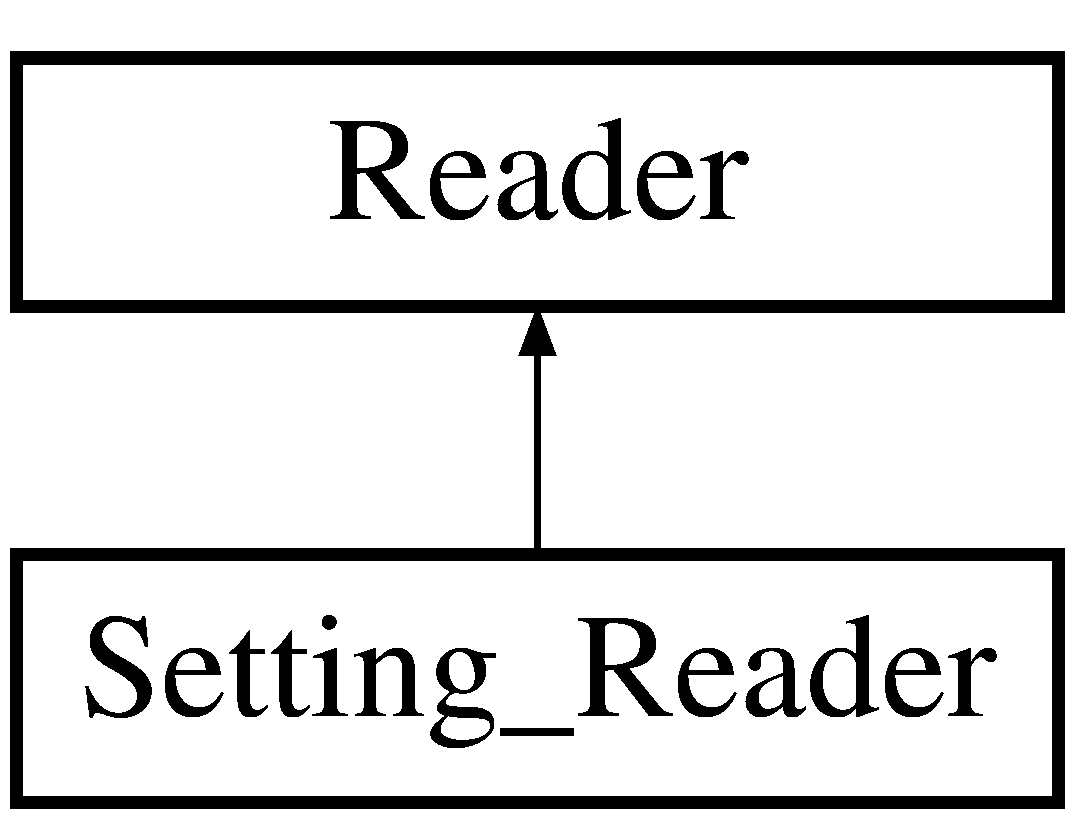
\includegraphics[height=2.000000cm]{class_setting___reader}
\end{center}
\end{figure}
\subsection*{Public Member Functions}
\begin{DoxyCompactItemize}
\item 
\mbox{\Hypertarget{class_setting___reader_a604a6eaadd0d39eb3d6b4ae768b95364}\label{class_setting___reader_a604a6eaadd0d39eb3d6b4ae768b95364}} 
\mbox{\hyperlink{class_setting___reader_a604a6eaadd0d39eb3d6b4ae768b95364}{Setting\+\_\+\+Reader}} (const string \&\mbox{\hyperlink{class_reader_a4f3eaccb117f248d4649ffb4e793a23d}{path}})
\begin{DoxyCompactList}\small\item\em Constructor. Initialize the attributes with the input argument. \end{DoxyCompactList}\item 
\mbox{\Hypertarget{class_setting___reader_a473c6649c848b28d53ebe99acb6f1c0f}\label{class_setting___reader_a473c6649c848b28d53ebe99acb6f1c0f}} 
\mbox{\hyperlink{struct_setting}{Setting}} \mbox{\hyperlink{class_setting___reader_a473c6649c848b28d53ebe99acb6f1c0f}{access\+\_\+setting}} () const
\begin{DoxyCompactList}\small\item\em Accessor. Provide access to the setting parameters. \end{DoxyCompactList}\item 
\mbox{\Hypertarget{class_setting___reader_a32f8f22c9ef67f4ab3f61f9cb5da69b3}\label{class_setting___reader_a32f8f22c9ef67f4ab3f61f9cb5da69b3}} 
void \mbox{\hyperlink{class_setting___reader_a32f8f22c9ef67f4ab3f61f9cb5da69b3}{read\+\_\+in}} () override
\begin{DoxyCompactList}\small\item\em Read the file from the path attribute and assign it to the setting attribute. \end{DoxyCompactList}\end{DoxyCompactItemize}
\subsection*{Protected Attributes}
\begin{DoxyCompactItemize}
\item 
\mbox{\Hypertarget{class_setting___reader_a5684da80f00261842f462606a1bfd5c8}\label{class_setting___reader_a5684da80f00261842f462606a1bfd5c8}} 
\mbox{\hyperlink{struct_setting}{Setting}} \mbox{\hyperlink{class_setting___reader_a5684da80f00261842f462606a1bfd5c8}{setting}}
\begin{DoxyCompactList}\small\item\em Attribute that stores the parameters read from the setting file. \end{DoxyCompactList}\end{DoxyCompactItemize}


\subsection{Detailed Description}
Inheritance of class \mbox{\hyperlink{class_reader}{Reader}} specialized in reading the setting file. 

The documentation for this class was generated from the following files\+:\begin{DoxyCompactItemize}
\item 
/\+Users/jiahuawu/\+Desktop/\+O\+D\+E\+\_\+\+Solver2/input.\+h\item 
/\+Users/jiahuawu/\+Desktop/\+O\+D\+E\+\_\+\+Solver2/input.\+cpp\end{DoxyCompactItemize}

\hypertarget{classtimesteppossitive}{}\section{timesteppossitive Class Reference}
\label{classtimesteppossitive}\index{timesteppossitive@{timesteppossitive}}


Inheritance of class exception\+: time step should not be negative or 0.  




{\ttfamily \#include $<$O\+D\+E\+\_\+solver.\+h$>$}

Inheritance diagram for timesteppossitive\+:\begin{figure}[H]
\begin{center}
\leavevmode
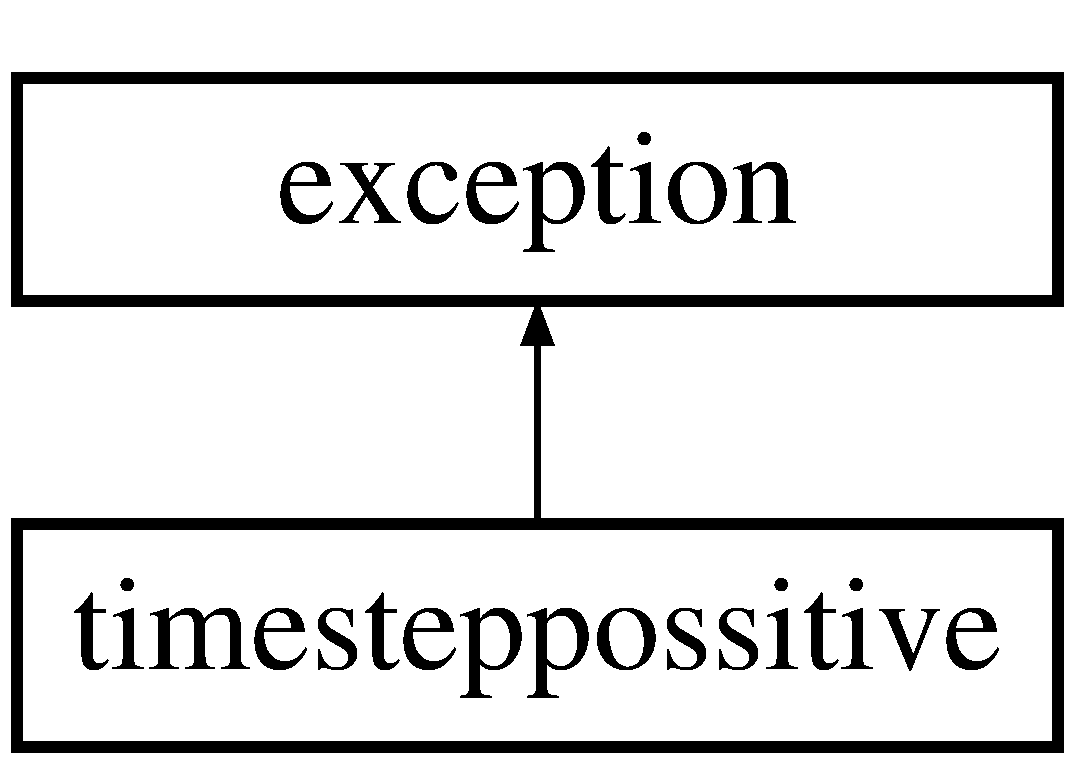
\includegraphics[height=2.000000cm]{classtimesteppossitive}
\end{center}
\end{figure}
\subsection*{Public Member Functions}
\begin{DoxyCompactItemize}
\item 
\mbox{\Hypertarget{classtimesteppossitive_acd3f5fd077ab556acf7f5abf73c87e3c}\label{classtimesteppossitive_acd3f5fd077ab556acf7f5abf73c87e3c}} 
virtual const char $\ast$ {\bfseries what} () const  throw ()
\end{DoxyCompactItemize}


\subsection{Detailed Description}
Inheritance of class exception\+: time step should not be negative or 0. 

The documentation for this class was generated from the following file\+:\begin{DoxyCompactItemize}
\item 
/\+Users/jiahuawu/\+Desktop/\+O\+D\+E\+\_\+\+Solver2/O\+D\+E\+\_\+solver.\+h\end{DoxyCompactItemize}

\hypertarget{class_vector___reader}{}\section{Vector\+\_\+\+Reader Class Reference}
\label{class_vector___reader}\index{Vector\+\_\+\+Reader@{Vector\+\_\+\+Reader}}


Inheritance of class \mbox{\hyperlink{class_data___reader}{Data\+\_\+\+Reader}} which specializes in reading files storing a vector.  




{\ttfamily \#include $<$Input.\+h$>$}

Inheritance diagram for Vector\+\_\+\+Reader\+:\begin{figure}[H]
\begin{center}
\leavevmode
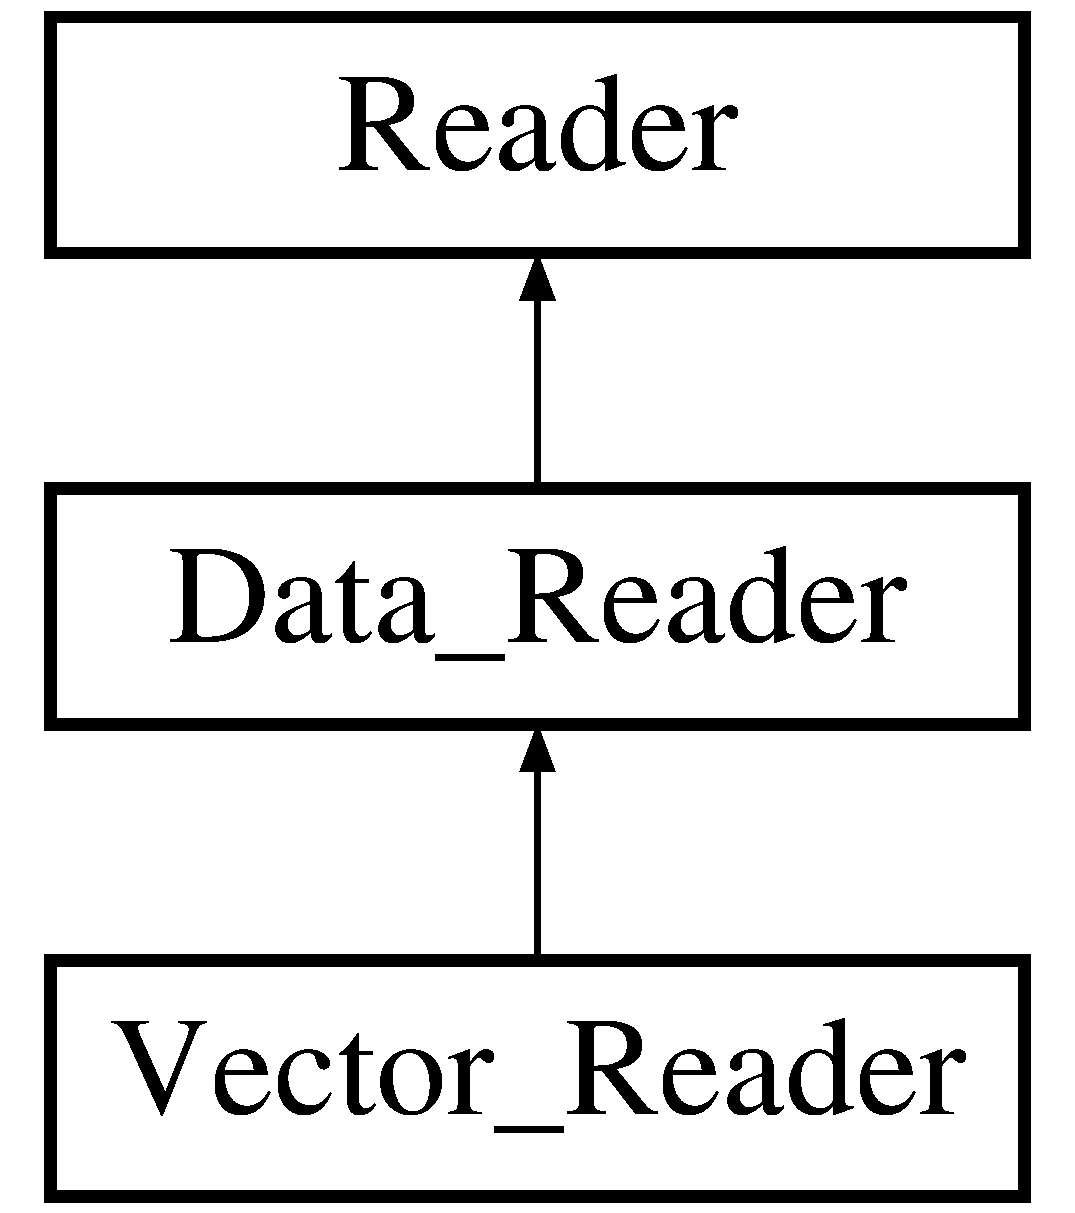
\includegraphics[height=3.000000cm]{class_vector___reader}
\end{center}
\end{figure}
\subsection*{Public Member Functions}
\begin{DoxyCompactItemize}
\item 
\mbox{\Hypertarget{class_vector___reader_a373565979af8b307dfddee36b22d7816}\label{class_vector___reader_a373565979af8b307dfddee36b22d7816}} 
\mbox{\hyperlink{class_vector___reader_a373565979af8b307dfddee36b22d7816}{Vector\+\_\+\+Reader}} (const string \&\mbox{\hyperlink{class_reader_a4f3eaccb117f248d4649ffb4e793a23d}{path}}, char \mbox{\hyperlink{class_data___reader_ac05700473d754089d7f30d2cc7dccce9}{delimiter}}=\textquotesingle{} \textquotesingle{})
\begin{DoxyCompactList}\small\item\em Constructor. Initialize data structure with the input arguments. \end{DoxyCompactList}\item 
\mbox{\Hypertarget{class_vector___reader_ad0609117e3120f06dda2eff01004f2be}\label{class_vector___reader_ad0609117e3120f06dda2eff01004f2be}} 
\mbox{\hyperlink{class_vector___reader_ad0609117e3120f06dda2eff01004f2be}{$\sim$\+Vector\+\_\+\+Reader}} () override
\begin{DoxyCompactList}\small\item\em Destructor. Deallocate the memory used by the vector attribute. \end{DoxyCompactList}\item 
\mbox{\Hypertarget{class_vector___reader_a60ca6034f26794cbc0a5acfbadf5cff4}\label{class_vector___reader_a60ca6034f26794cbc0a5acfbadf5cff4}} 
Vector \mbox{\hyperlink{class_vector___reader_a60ca6034f26794cbc0a5acfbadf5cff4}{access\+\_\+vector}} () const
\begin{DoxyCompactList}\small\item\em Accessor. Access the vector read from the file. \end{DoxyCompactList}\item 
\mbox{\Hypertarget{class_vector___reader_aa4ce4311cab6358f17813bb293456942}\label{class_vector___reader_aa4ce4311cab6358f17813bb293456942}} 
void \mbox{\hyperlink{class_vector___reader_aa4ce4311cab6358f17813bb293456942}{read\+\_\+in}} () override
\begin{DoxyCompactList}\small\item\em Read the file from the path attribute and assign it to the vector attribute. \end{DoxyCompactList}\end{DoxyCompactItemize}
\subsection*{Protected Attributes}
\begin{DoxyCompactItemize}
\item 
\mbox{\Hypertarget{class_vector___reader_a9b12a16c14096fd15f2c32f0afbb3b53}\label{class_vector___reader_a9b12a16c14096fd15f2c32f0afbb3b53}} 
Vector \mbox{\hyperlink{class_vector___reader_a9b12a16c14096fd15f2c32f0afbb3b53}{y}}
\begin{DoxyCompactList}\small\item\em Vector read from the file. \end{DoxyCompactList}\end{DoxyCompactItemize}


\subsection{Detailed Description}
Inheritance of class \mbox{\hyperlink{class_data___reader}{Data\+\_\+\+Reader}} which specializes in reading files storing a vector. 

The documentation for this class was generated from the following files\+:\begin{DoxyCompactItemize}
\item 
/\+Users/jiahuawu/\+Desktop/\+O\+D\+E\+\_\+\+Solver/include/Input.\+h\item 
/\+Users/jiahuawu/\+Desktop/\+O\+D\+E\+\_\+\+Solver/src/Input.\+cpp\end{DoxyCompactItemize}

%--- End generated contents ---

% Index
\backmatter
\newpage
\phantomsection
\clearemptydoublepage
\addcontentsline{toc}{chapter}{Index}
\printindex

\end{document}
